\documentclass[pdflatex,sn-mathphys-num]{sn-jnl}

%%%% --------------------------------------------------------------------
%%%% PACKAGES
%%%% --------------------------------------------------------------------
% sn-jnl natively loads graphicx, amsmath, xcolor, etc., but declaring them 
% here is safe. Removed conflicting packages (titlesec, caption, float).
\usepackage{graphicx}
\usepackage{multirow}
\usepackage{amsmath,amssymb,amsfonts}
\usepackage{amsthm}
\usepackage{mathrsfs}
\usepackage[title]{appendix}
\usepackage{xcolor}
\usepackage{textcomp}
\usepackage{manyfoot}
\usepackage{booktabs}
\usepackage{algorithm}
\usepackage{algorithmicx}
\usepackage{algpseudocode}
\usepackage{listings}
\usepackage{tikz}
\usepackage{microtype}

%%%% --------------------------------------------------------------------
%%%% TIKZ CONFIGURATION
%%%% --------------------------------------------------------------------
\usetikzlibrary{positioning, arrows.meta, shapes.geometric, fit, backgrounds}

%%%% --------------------------------------------------------------------
%%%% MATH & THEOREMS
%%%% --------------------------------------------------------------------
\DeclareMathOperator*{\argmax}{arg\,max}

\theoremstyle{thmstyleone}
\newtheorem{theorem}{Theorem}
\newtheorem{proposition}[theorem]{Proposition}

\theoremstyle{thmstyletwo}
\newtheorem{example}{Example}
\newtheorem{remark}{Remark}

\theoremstyle{thmstylethree}
\newtheorem{definition}{Definition}

%%%% --------------------------------------------------------------------
%%%% TYPOGRAPHY FIXES (STRICT)
%%%% --------------------------------------------------------------------
\widowpenalty=10000
\clubpenalty=10000
\displaywidowpenalty=10000
\emergencystretch=3em

\begin{document}

\title[CLAFPP++: Calibrated Neuro-Symbolic Ensemble for NIDS]{CLAFPP++: A Calibrated Neuro-Symbolic Ensemble for Interpretable Network Intrusion Detection}

\author*[1]{\fnm{Nirzor} \sur{Chowdhury}}\email{nirzor.chy10@gmail.com}

\author[1]{\fnm{Sandeep} \sur{Gurung}}\email{sandeep.g@smit.smu.edu.in}

\affil*[1]{\orgdiv{Department of Computer Science and Engineering}, \orgname{Sikkim Manipal Institute of Technology, Sikkim Manipal University}, \orgaddress{\city{Majitar}, \state{Sikkim}, \country{India}}}

\abstract{There is growing pressure on network intrusion detection systems (NIDSs) to provide high detection performance while maintaining interpretability for security analysts who have to act upon their outputs. Although stacked ensemble methods frequently yield uncalibrated outputs and depend on post-hoc techniques for explainability, they have demonstrated encouraging outcomes on benchmark datasets. CLAFPP++, a calibrated stacked neuro-symbolic ensemble for binary intrusion detection, is presented in this paper. Through a calibrated logistic-regression meta-learner with a residual symbolic enhancer trained on a held-out calibration split, the framework combines five expert branches: a generative branch that combines an autoencoder and a GANomaly model, a sequence-style BiLSTM, a one-dimensional convolutional model, a tree-based learner, and a data-driven symbolic rule engine. Using paired statistical tests, we assess CLAFPP++ on NSL-KDD and Edge-IIoTset across five random seeds and compare it to a tailored XGBoost baseline trained on identical splits. At a false-alarm rate of $0.080 \pm 0.011$, CLAFPP++ obtains $\mathrm{AUROC} = 0.963 \pm 0.001$ and $\mathrm{AUPRC} = 0.965 \pm 0.003$ on NSL-KDD. These results are statistically indistinguishable on $F_1$ from an adjusted XGBoost baseline ($p = 0.486$, Cohen's $d = 0.34$). On Edge-IIoTset, CLAFPP++ obtains $F_1 = 0.995 \pm 0.001$ at a false-alarm rate of $0.0009$ following an explicit leakage audit that eliminates six artificially separated characteristics. The symbolic layer supports per-prediction explainability without compromising discrimination performance by generating per-rule attributions with up to $1.000$ standalone precision. We present the results of the leakage audit and suggest that future research should focus on dataset-specific symbolic rule construction.}

\keywords{Anomaly detection, Calibration, Ensemble learning, Interpretability, Intrusion detection, Network security, Neuro-symbolic learning}

\maketitle

\section{Introduction}\label{sec:intro}

Network intrusion detection systems (NIDSs) remain a critical line of defence in modern enterprise and industrial networks. As traffic volumes grow and attack patterns become more diverse, NIDSs face increasing pressure to deliver high detection performance while remaining interpretable to the security analysts who must act on their outputs. A NIDS that flags an alert without exposing the basis for that alert places the entire interpretive burden on the analyst, a cost that is particularly acute in environments where alert volume is already a known operational concern~\cite{shone2017deep,gurung2019deep}.

A substantial body of recent work has explored ensemble learning for NIDS, in which the outputs of multiple base classifiers are combined to improve robustness and discrimination. Stacking, in which a meta-learner is trained on the predictions of the base classifiers, has become a particularly popular formulation~\cite{infuse2023,eed2024,ji2025stacked}. Such approaches have demonstrated promising results on benchmark datasets, often matching or surpassing single-classifier baselines. However, two limitations of the current ensemble-based NIDS literature motivate the present work.

First, many stacked-ensemble approaches treat the meta-learner as a black box and report only point predictions or uncalibrated scores. Probability calibration---ensuring that a predicted score of $0.9$ corresponds to a true positive rate of approximately $90\%$---is rarely audited, yet it is essential for downstream decision-making such as threshold tuning, alert ranking, and human-in-the-loop triage. Without calibration, the meta-learner's outputs cannot be reliably composed with operational policies.

Second, interpretability in ensemble NIDSs is typically addressed post hoc, often through feature-importance tools applied to the base classifiers or the meta-learner. Such tools can be informative but do not yield analyst-facing explanations that connect a prediction to recognizable attack signatures. A complementary line of work has examined symbolic and neuro-symbolic approaches, in which hand-designed or data-driven rules encode known attack patterns alongside neural components~\cite{neurosymbolic2025iot,neurosymbolic2026sensors}. These approaches retain the explanatory power of rule-based systems while benefiting from the representational capacity of neural models. However, where the symbolic component is reported to contribute to discrimination, the contribution is often modest, and the interpretability claim is not always supported by per-prediction case studies or per-rule statistical evidence.

This paper introduces CLAFPP++ (Conditional Latent Anomaly Fusion with Probabilistic Propagation), a calibrated stacked neuro-symbolic ensemble for binary network intrusion detection. The framework combines five expert branches that capture complementary views of network traffic---a generative branch combining an autoencoder and a GANomaly model, a sequence model, a one-dimensional convolutional model, a tree-based classifier, and a data-driven symbolic rule engine---through a calibrated logistic-regression meta-learner. A residual symbolic enhancer adjusts the final prediction using rule activations, and its weighting parameter $\lambda$ is fit on a held-out subset of the validation data, separate from the data used to train the meta-learner, to mitigate optimization on saturated signals.

We evaluate CLAFPP++ on two heterogeneous benchmark datasets. NSL-KDD~\cite{tavallaee2009detailed} remains the most widely-used corpus for direct comparison with prior NIDS work and supports comparability with the broader literature. Edge-IIoTset~\cite{ferrag2022edge} is a more recent dataset that reflects modern Internet-of-Things and Industrial-Internet-of-Things traffic, including attack families that are absent from NSL-KDD. We additionally report an explicit data-leakage audit on Edge-IIoTset, in which a small number of features with near-perfect single-feature separability with the target label are identified and removed prior to all experiments. This audit, which to the best of our knowledge has not been systematically reported in prior Edge-IIoTset work, brings the headline numbers in line with what we believe to be a more honest baseline for the dataset.

This paper offers the following novel contributions:
\begin{enumerate}
    \item A calibrated stacked neuro-symbolic ensemble architecture for binary network intrusion detection, in which five expert branches are fused through a calibrated logistic-regression meta-learner with a residual symbolic enhancer trained on a held-out calibration split, an arrangement that mitigates optimization on saturated validation signals.
    \item An evaluation protocol that reports performance across five random seeds with paired statistical-significance testing (paired $t$-test, Wilcoxon signed-rank, and Cohen's $d$ effect sizes), together with a tuned single-classifier baseline (XGBoost) trained on the same data splits, for direct apples-to-apples comparison.
    \item A symbolic interpretability analysis comprising per-rule global statistics on the test set (standalone precision and recall when each rule is used as an independent classifier) and per-prediction case studies that demonstrate the rule activations underlying selected true-positive and false-negative predictions.
    \item An explicit data-leakage audit on Edge-IIoTset that identifies and removes features inducing artificial separability with the target label, accompanied by a discussion of the implications for cross-paper comparability on this dataset.
\end{enumerate}

The remainder of this paper is organized as follows. Section~\ref{sec:background} provides background on the techniques used in our framework. Section~\ref{sec:related} surveys related work in stacked-ensemble and neuro-symbolic NIDSs. Section~\ref{sec:method} details the proposed CLAFPP++ architecture. Section~\ref{sec:setup} describes the experimental setup, including datasets, preprocessing, and the Edge-IIoTset leakage audit. Section~\ref{sec:results} presents results on both datasets, including statistical-significance analysis and the symbolic interpretability case studies. Section~\ref{sec:discussion} discusses the findings, with particular attention to the conditions under which the symbolic residual enhancer contributes interpretive value rather than discrimination gain. Section~\ref{sec:conclusion} concludes and outlines future work.

\section{Background}\label{sec:background}

This section provides background on the techniques used in CLAFPP++. The aim is to introduce the concepts at a level sufficient for a reader unfamiliar with each individual component; readers familiar with these techniques may proceed to Section~\ref{sec:related}.

\subsection{Network Intrusion Detection}
A NIDS examines network traffic, typically represented as connection records or packet flows, and assigns each record a label indicating whether it is consistent with normal activity or with an attack pattern~\cite{shone2017deep,tavallaee2009detailed}. In the binary formulation considered in this paper, the label is either \emph{normal} or \emph{attack}; multi-class formulations that distinguish among attack families are also common but lie outside the scope of this work. A NIDS is typically evaluated on accuracy, precision, recall, the harmonic mean of precision and recall (the $F_1$ score), the false alarm rate, and the area under the receiver operating characteristic curve (AUROC). The false alarm rate is particularly important from a deployment perspective: even modest values, when applied to high-volume traffic, can produce alert workloads that exceed the capacity of human analysts.

\subsection{Autoencoders and the Generative Branch}
An autoencoder is an unsupervised neural network trained to reconstruct its input through a lower-dimensional bottleneck. The model learns parameters $\theta = (W, b)$ that minimize a reconstruction loss $\mathcal{L}(x, \hat{x})$, where $\hat{x}$ is the network's output and $x$ is the input. For anomaly detection, the autoencoder is trained predominantly on benign traffic; samples that the trained model reconstructs poorly are flagged as candidate anomalies, on the assumption that reconstruction quality reflects similarity to the training distribution.

GANomaly~\cite{akcay2019ganomaly} extends this idea by combining an autoencoder with an adversarial training scheme. A discriminator is trained to distinguish reconstructed samples from real ones, and an additional encoder maps the reconstructed sample back into the latent space. The anomaly score combines reconstruction error, latent-space distance, and adversarial feedback. The two models capture complementary signals: the autoencoder is sensitive to reconstruction failures, while GANomaly is sensitive to distributional shifts in the latent space. In CLAFPP++ we treat these two outputs as a single \emph{generative branch} and fuse them before passing to the meta-learner.

\subsection{Sequence and Pattern Models for Tabular Network Records}
NSL-KDD and Edge-IIoTset both supply tabular per-connection records rather than packet-level time series. We include a bi-directional long short-term memory (BiLSTM) model and a one-dimensional convolutional model in our framework as complementary feature mixers: the BiLSTM captures interactions across feature positions, while the convolutional model captures local patterns. We treat the temporal interpretation of the BiLSTM with care: NSL-KDD records do not carry an authoritative temporal ordering, so we use the model as a feature mixer rather than as a sequence model in the strict sense.

\subsection{Tree Ensembles and Calibration}
Random Forest and gradient-boosted trees, particularly XGBoost~\cite{chen2016xgboost}, are widely used in tabular intrusion detection and are competitive on both NSL-KDD and Edge-IIoTset. Tree ensembles produce well-separated decision boundaries but are not inherently calibrated: their raw scores may not correspond to true posterior probabilities. Calibration techniques such as Platt scaling and isotonic regression~\cite{platt1999probabilistic,niculescu2005predicting} adjust the score distribution to better approximate true probabilities. Calibration is particularly relevant in stacked ensembles, where the meta-learner consumes the outputs of multiple base classifiers; uncalibrated inputs can mislead the meta-learner about the relative confidence of its components.

\subsection{Symbolic and Neuro-Symbolic Components}
Symbolic systems encode attack patterns as rules over features, often using thresholds, conjunctions, and disjunctions designed by domain experts or derived from data~\cite{neurosymbolic2025iot}. Such systems produce predictions that are transparent in the sense that the rule activations underlying a prediction can be inspected directly. Neuro-symbolic systems combine symbolic reasoning with neural components, typically using the neural model for representation learning and the symbolic system either as a constraint, an interpretive overlay, or a residual adjustment to the neural prediction. In CLAFPP++ the symbolic engine plays the third role: it adjusts the neural meta-learner's output by a learned weighting $\lambda$, supports per-prediction explanations through rule activations, and is fit on data the meta-learner does not see during training.

\section{Related Work}\label{sec:related}

We organize the related work into three subsections: stacked-ensemble NIDSs, neuro-symbolic and explainable NIDSs, and the broader use of the Edge-IIoTset benchmark. Throughout, we cite recent work (2022--2026) where comparable approaches have been reported, and we situate CLAFPP++ relative to each line of research.

\subsection{Stacked-Ensemble NIDSs}
Stacked ensembles have become a popular family of approaches for tabular network-intrusion detection, motivated by the observation that no single classifier consistently dominates across attack families. Mills~\textit{et al.}~\cite{mills2024hybrid} present a hybrid IDS that combines a multilayer perceptron, a modified self-organizing map, and a decision tree as base learners, with a J48 decision tree serving as the meta-learner, and report results on NSL-KDD and CIC-DDoS2019. Ji~\textit{et al.}~\cite{ji2025stacked} propose a meta-learning framework for cyber-physical systems that uses random forest, gradient boosting, multilayer perceptron, and $k$-nearest neighbors as base classifiers with an XGBoost meta-learner, supported by an autoencoder for feature selection; the authors report accuracies above $98\%$ on both CIC-IoT-2023 and NSL-KDD. Khan~\textit{et al.}~\cite{khan2024robust} stack multiple deep-learning base models on NSL-KDD, and Ahmad~\textit{et al.}~\cite{ahmad2024automl} apply an AutoML-driven stacked ensemble to the same benchmark, reporting accuracies around $90\%$. Rashid~\textit{et al.}~\cite{rashid2022twostage} present SE-IDS, which uses five tree-based base learners (decision tree, XGBoost, bagging, extra trees, random forest) with a multilayer perceptron meta-learner. More recently, autonomous multi-layered stacking frameworks with dynamic feature subset optimization have been proposed for general-purpose intrusion detection~\cite{bah2025autonomous}.

These approaches share three structural traits with the present work: a heterogeneous base-classifier pool, a trained meta-learner, and an emphasis on tabular benchmark datasets such as NSL-KDD. However, none of the works cited above audit the calibration of the meta-learner's output probabilities, and few report per-seed variance with paired statistical tests. Earlier work from our research group~\cite{gurung2019deep} applied deep-learning techniques to the NSL-KDD dataset and helped motivate the present extension toward calibrated stacked architectures with symbolic interpretability companions. Comprehensive ensemble pipelines such as INFUSE~\cite{infuse2023} similarly motivate fused base-classifier approaches, though their primary emphasis is on representational fusion rather than per-prediction interpretability.

\subsection{Neuro-Symbolic and Explainable NIDSs}
Explainability in NIDSs is most commonly addressed through post-hoc attribution tools such as SHAP and LIME applied to a trained classifier~\cite{grabowski2025explainable,xai2025engapps}. The Explainable Ensemble Deep-learning method of Ben Ncir~\textit{et al.}~\cite{eed2024} combines a long short-term memory-based ensemble with SHAP-based interpretation, and is among the closest prior approaches to CLAFPP++ in spirit: both works aim to deliver interpretable ensemble-based intrusion detection. The principal difference is that the cited approach uses SHAP as a post-hoc attribution layer applied to neural outputs, while CLAFPP++ integrates symbolic rules as a first-class component of the ensemble whose activations are themselves the explanations.

A more recent line of research investigates neuro-symbolic intrusion detection, in which symbolic reasoning is combined with neural representation learning. Sai~\textit{et al.}~\cite{sai2025neurosymbolic} present a dual-model neuro-symbolic architecture for explainable and resilient intrusion detection in IoT networks, evaluated on the NF-BoT-IoT-V2 dataset. Akhter~\textit{et al.}~\cite{akhter2025neurosymbolic} discuss neuro-symbolic frameworks for IoT-driven smart-city applications more broadly, including security use cases. Most recently, Kalutharage~\textit{et al.}~\cite{neurosymbolic2026sensors} propose a lightweight neuro-symbolic edge-IDS framework that integrates neural learning, symbolic rule-based reasoning, and knowledge distillation for real-time deployment, evaluated on Edge-IIoTset.

These neuro-symbolic approaches typically pursue one of two goals: either to use symbolic structure as a regularizer or constraint on neural learning, or to produce human-readable explanations that complement neural predictions. The interpretability claim in much of the cited literature is supported primarily by architectural arguments or qualitative examples; quantitative per-rule statistics (such as the standalone precision and recall of each rule when used as an independent classifier) are reported less consistently. In CLAFPP++, we treat such quantitative per-rule statistics as an explicit evaluation product alongside the headline detection numbers.

\subsection{The Edge-IIoTset Benchmark}
Edge-IIoTset was introduced by Ferrag~\textit{et al.}~\cite{ferrag2022edge} as a comprehensive realistic dataset of IoT and IIoT applications, collected from a purpose-built testbed with multiple devices, sensors, and protocols. The dataset has been adopted widely in subsequent work, including comparative IDS evaluations~\cite{tareq2023comparative}, federated-learning studies, and the neuro-symbolic edge framework cited above~\cite{neurosymbolic2026sensors}. Reported binary-classification performance on Edge-IIoTset is generally high---above $99\%$ accuracy in many studies---when standard preprocessing is applied. As part of the present work, we observe that a small set of categorically-encoded protocol-specific features in the dataset exhibit near-perfect single-feature separability with the target label, an artifact of how categorical strings were assigned during preparation. We discuss this finding and our leakage-correction protocol in Section~\ref{sec:setup}.

\subsection{Positioning of CLAFPP++}
CLAFPP++ contributes to the stacked-ensemble and neuro-symbolic NIDS literature in four respects. First, the meta-learner is a calibrated logistic-regression model with its calibration audited rather than assumed. Second, the symbolic component is integrated as a learned residual whose weighting parameter $\lambda$ is fit on a held-out validation subset, mitigating the saturation-on-validation effects that we believe underlie some of the modest symbolic-contribution numbers reported in prior neuro-symbolic IDS work. Third, the symbolic component is evaluated quantitatively at the per-rule level on the test set, in addition to the standard ensemble-level metrics. Fourth, we report multi-seed performance with paired statistical tests, a tuned single-classifier (XGBoost) baseline, and a data-leakage audit on Edge-IIoTset, in order to support apples-to-apples comparison with future work on the same benchmarks.

\section{Proposed Methodology}\label{sec:method}

This section presents the proposed CLAFPP++ framework. Section~\ref{sec:method-overview} describes the overall architecture. Section~\ref{sec:method-branches} details the five expert branches. Section~\ref{sec:method-meta} describes the stacked meta-learner and its calibration. Section~\ref{sec:method-symbolic} formalizes the residual symbolic enhancer. Section~\ref{sec:method-threshold} specifies the threshold-selection protocol used for all reported metrics.

\subsection{Architecture Overview}\label{sec:method-overview}

CLAFPP++ is a binary classifier that maps a network connection record $x \in \mathbb{R}^{d}$ to a probability $p(y=1 \mid x) \in [0,1]$ that the record corresponds to an attack. The architecture is illustrated in Fig.~\ref{fig:arch}. Five expert branches operate in parallel on a preprocessed feature representation of $x$: a generative branch combining an autoencoder and a GANomaly model, a sequence-style branch based on a bi-directional long short-term memory (BiLSTM) network, a pattern-style branch based on a one-dimensional convolutional neural network (1D-CNN), a tabular branch combining a random forest and an XGBoost classifier through soft averaging, and a symbolic branch that produces an aggregate rule-engine score. The five branch outputs are concatenated into a meta-feature vector and augmented with simple summary statistics (per-sample minimum, maximum, mean, standard deviation, and disagreement). A calibrated logistic-regression meta-learner is then trained on the meta-feature vector to produce a primary neural meta score $s_{\mathrm{meta}}(x)$. A residual symbolic enhancer adjusts this score by a learned weighting $\lambda$ of the normalized symbolic-engine score, yielding the final CLAFPP++ score
\begin{equation}
\label{eq:final-score}
s_{\mathrm{CLAFPP++}}(x) = \mathrm{clip}\!\left( s_{\mathrm{meta}}(x) + \lambda \cdot \tilde{r}(x),\, 0,\, 1 \right),
\end{equation}
where $\tilde{r}(x)$ is the normalized symbolic score (defined in Section~\ref{sec:method-symbolic}) and $\mathrm{clip}(\cdot, 0, 1)$ denotes elementwise clipping to the unit interval. A binary prediction is obtained by thresholding $s_{\mathrm{CLAFPP++}}(x)$ at a value $\tau \in [0,1]$ selected as described in Section~\ref{sec:method-threshold}.

\begin{figure}[!ht]
\centering
\resizebox{\textwidth}{!}{%
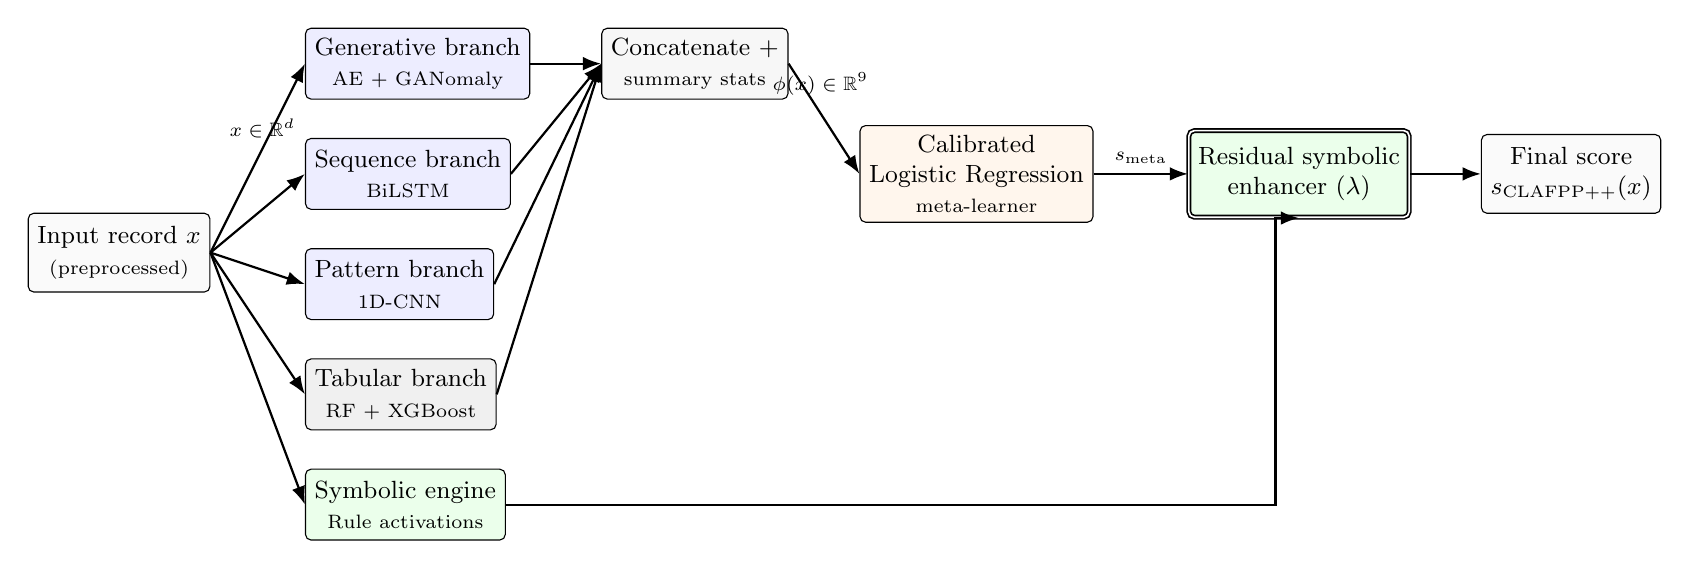
\begin{tikzpicture}[
    node distance=3mm and 6mm,
    every node/.style={font=\small},
    % soft blue for neural branches
    neural/.style={draw, rounded corners=2pt, minimum width=22mm, minimum height=9mm,
                   align=center, fill=blue!7},
    % light gray for the tabular branch
    tabular/.style={draw, rounded corners=2pt, minimum width=22mm, minimum height=9mm,
                    align=center, fill=black!6},
    % soft green for symbolic components
    symb/.style={draw, rounded corners=2pt, minimum width=22mm, minimum height=9mm,
                 align=center, fill=green!8},
    % fusion component (meta-learner): neutral tint
    meta/.style={draw, rounded corners=2pt, minimum width=28mm, minimum height=10mm,
                 align=center, fill=orange!7},
    % novel component: thicker double border to draw the reader's eye
    enhancer/.style={draw, double, line width=0.6pt, rounded corners=2pt,
                     minimum width=26mm, minimum height=11mm, align=center, fill=green!8},
    sumbox/.style={draw, rounded corners=2pt, minimum width=22mm, minimum height=9mm,
                   align=center, fill=black!3},
    inout/.style={draw, rounded corners=2pt, minimum width=22mm, minimum height=10mm,
                  fill=black!2, align=center},
    arrow/.style={-Latex, thick},
    dimlabel/.style={font=\scriptsize}
]

\node[inout] (input) {Input record $x$\\\scriptsize (preprocessed)};

\node[neural,  right=12mm of input, yshift=24mm] (gen) {Generative branch\\\scriptsize AE + GANomaly};
\node[neural,  right=12mm of input, yshift=10mm] (seq) {Sequence branch\\\scriptsize BiLSTM};
\node[neural,  right=12mm of input, yshift=-4mm] (cnn) {Pattern branch\\\scriptsize 1D-CNN};
\node[tabular, right=12mm of input, yshift=-18mm] (tab) {Tabular branch\\\scriptsize RF + XGBoost};
\node[symb,    right=12mm of input, yshift=-32mm] (sym) {Symbolic engine\\\scriptsize Rule activations};

\node[sumbox, right=9mm of gen] (concat) {Concatenate +\\\scriptsize summary stats};

\node[meta, right=9mm of concat, yshift=-14mm] (metalrn) {Calibrated\\Logistic Regression\\\scriptsize meta-learner};

\node[enhancer, right=12mm of metalrn] (enhancer) {Residual symbolic\\enhancer ($\lambda$)};

\node[inout, right=9mm of enhancer] (out) {Final score\\$s_{\mathrm{CLAFPP++}}(x)$};

\draw[arrow] (input.east) -- node[dimlabel, pos=0.55, above] {$x \in \mathbb{R}^{d}$} (gen.west);
\draw[arrow] (input.east) -- (seq.west);
\draw[arrow] (input.east) -- (cnn.west);
\draw[arrow] (input.east) -- (tab.west);
\draw[arrow] (input.east) -- (sym.west);

\draw[arrow] (gen.east) -- (concat.west);
\draw[arrow] (seq.east) -- (concat.west);
\draw[arrow] (cnn.east) -- (concat.west);
\draw[arrow] (tab.east) -- (concat.west);

\draw[arrow] (concat.east) -- node[dimlabel, pos=0.45, above=1mm] {$\phi(x)\in\mathbb{R}^{9}$} (metalrn.west);
\draw[arrow] (metalrn.east) -- node[dimlabel, pos=0.5, above] {$s_{\mathrm{meta}}$} (enhancer.west);
\draw[arrow] (sym.east) -| ([xshift=-3mm]enhancer.south) -- (enhancer.south);
\draw[arrow] (enhancer.east) -- (out.west);

\end{tikzpicture}%
}
\caption{Architecture of the CLAFPP++ framework. Five expert branches are grouped by
learning paradigm: neural branches (generative, sequence, pattern; light blue), the
tabular branch (gray), and the symbolic engine (green). The four neural and tabular
branch outputs are concatenated with summary statistics into a nine-dimensional
meta-feature vector $\phi(x)$ and passed to a calibrated logistic-regression
meta-learner. The residual symbolic enhancer (double border, our principal
architectural contribution) adjusts the meta-learner's output $s_{\mathrm{meta}}$ by
a learned weighting $\lambda$ of the normalized symbolic-engine score.}
\label{fig:arch}
\end{figure}

\subsection{Expert Branches}\label{sec:method-branches}

\subsubsection{Generative Branch}
The generative branch combines an autoencoder with a GANomaly model~\cite{akcay2019ganomaly}, each trained predominantly on benign traffic. The autoencoder produces a reconstruction-error score $g_{\mathrm{AE}}(x)$; the GANomaly model produces a hybrid score $g_{\mathrm{GAN}}(x)$ that combines reconstruction error, latent-space distance, and discriminator feedback. The two scores are fused as
\begin{equation}
\label{eq:gen-fusion}
g(x) = w_{\mathrm{AE}} \cdot g_{\mathrm{AE}}(x) + w_{\mathrm{GAN}} \cdot g_{\mathrm{GAN}}(x),
\end{equation}
where $w_{\mathrm{AE}}, w_{\mathrm{GAN}} \in [0,1]$ with $w_{\mathrm{AE}} + w_{\mathrm{GAN}} = 1$, and both weights are constrained to lie above a configurable floor to prevent any single sub-model from dominating the branch output. Both sub-models receive standardized input.

\subsubsection{Sequence Branch (BiLSTM)}
The sequence branch is a bi-directional long short-term memory network operating over the standardized feature vector. As noted in Section~\ref{sec:background}, the NSL-KDD records do not carry an authoritative temporal ordering, and we treat the BiLSTM as a feature mixer rather than as a temporal model in the strict sense. Its output is the probability assigned to the positive (attack) class.

\subsubsection{Pattern Branch (1D-CNN)}
The pattern branch is a one-dimensional convolutional neural network with a small number of channels and a single fully-connected output head. Convolutional kernels span subsets of adjacent feature positions, capturing local interactions among features in the preprocessed representation. The output is again the probability assigned to the positive class.

\subsubsection{Tabular Branch}
The tabular branch combines a random forest classifier and an XGBoost classifier~\cite{chen2016xgboost} via soft averaging:
\begin{equation}
\label{eq:tab-fusion}
t(x) = w_{\mathrm{RF}} \cdot t_{\mathrm{RF}}(x) + w_{\mathrm{XGB}} \cdot t_{\mathrm{XGB}}(x),
\end{equation}
where the weights are constrained by the same weight-floor mechanism as in~\eqref{eq:gen-fusion}. Both sub-models are trained on the min--max-scaled feature vector with class-balanced weighting; XGBoost is configured with histogram-based tree construction for training efficiency.

\subsubsection{Symbolic Branch}
The symbolic branch is a rule engine in which each rule is a function $r_k(x) \in [0,1]$ of selected features that returns a confidence score for the rule's activation. The rule definitions are dataset-specific: on NSL-KDD they encode classical NIDS signatures (for example, SYN-flood-consistency patterns and service-sweep dispersion); on Edge-IIoTset they encode IoT-protocol-specific signatures (for example, DDoS flag storms and HTTP request anomalies). Each rule is associated with a learned weight $\omega_k$ obtained from a fitting procedure on the training set, subject to a configurable weight floor to prevent any single rule from being suppressed entirely. The aggregate symbolic score is
\begin{equation}
\label{eq:sym-aggregate}
r(x) = \sum_{k=1}^{K} \omega_k \, r_k(x), \qquad \sum_{k=1}^{K} \omega_k = 1.
\end{equation}
The individual rule activations $\{r_k(x)\}_{k=1}^{K}$ are retained in addition to the aggregate score $r(x)$, since they constitute the per-prediction explanations evaluated in Section~\ref{sec:results}.

\subsection{Stacked Meta-Learner with Calibration}\label{sec:method-meta}

The four neural and tabular branch outputs $\{g(x), \ell(x), c(x), t(x)\}$, where $\ell(x)$ and $c(x)$ denote the BiLSTM and 1D-CNN outputs respectively, are concatenated and augmented with five summary statistics computed across the four scores: minimum, maximum, mean, standard deviation, and disagreement (the range $\max - \min$). The resulting nine-dimensional meta-feature vector $\phi(x) \in \mathbb{R}^{9}$ is the input to the meta-learner.

The meta-learner is a logistic-regression classifier $M_\theta$ trained on $\phi(x)$. We use logistic regression rather than a deeper or higher-capacity model for two reasons. First, the dimensionality of $\phi(x)$ is small (nine) and the number of training examples available to the meta-learner is on the order of $10^{4}$, so a high-capacity meta-learner is prone to overfit the validation pool on which it is trained. Second, logistic regression produces probability outputs whose calibration can be audited directly and adjusted with standard tools such as Platt scaling~\cite{platt1999probabilistic} when necessary.

To prevent the meta-learner from optimizing on validation signals that are subsequently consumed by the symbolic enhancer, we partition the validation pool $\mathcal{V}$ into a meta-training subset $\mathcal{V}_{\mathrm{m}}$ and a calibration/enhancer subset $\mathcal{V}_{\mathrm{c}}$, with $|\mathcal{V}_{\mathrm{m}}| = 0.6 \cdot |\mathcal{V}|$ and $|\mathcal{V}_{\mathrm{c}}| = 0.4 \cdot |\mathcal{V}|$, stratified by class. The meta-learner is trained on $\mathcal{V}_{\mathrm{m}}$ only. Feature standardization parameters for $\phi$ are estimated from $\mathcal{V}_{\mathrm{m}}$ and applied to $\mathcal{V}_{\mathrm{c}}$ and to the test set. The trained meta-learner produces the neural meta score
\begin{equation}
\label{eq:meta-score}
s_{\mathrm{meta}}(x) = M_\theta\!\left( \phi(x) \right).
\end{equation}

\subsection{Residual Symbolic Enhancer}\label{sec:method-symbolic}

The residual symbolic enhancer combines the neural meta score $s_{\mathrm{meta}}$ with the symbolic-engine score $r$ through a learned residual weighting. We first normalize the raw symbolic score so that it lies on a comparable scale to the meta score. Let $\mu_r$ and $\sigma_r$ denote the mean and standard deviation of $r(x)$ over the calibration subset $\mathcal{V}_{\mathrm{c}}$. The normalized symbolic score is
\begin{equation}
\label{eq:sym-normalize}
\tilde{r}(x) = \sigma\!\left( \frac{r(x) - \mu_r}{\sigma_r + \epsilon} \right),
\end{equation}
where $\sigma(\cdot)$ denotes the logistic sigmoid and $\epsilon$ is a small positive constant for numerical stability. The parameters $\mu_r$ and $\sigma_r$ are stored after fitting and re-applied at inference time, so that training-time and inference-time normalization are identical.

The weighting $\lambda$ is selected by grid search over a discrete set $\Lambda \subset [0, \lambda_{\max}]$ to maximize the area under the precision--recall curve (AUPRC) on $\mathcal{V}_{\mathrm{c}}$:
\begin{equation}
\label{eq:lambda-objective}
\lambda^{\star} = \argmax_{\lambda \in \Lambda} \mathrm{AUPRC}\!\left( y^{(\mathrm{c})},\, \mathrm{clip}(s_{\mathrm{meta}}^{(\mathrm{c})} + \lambda \cdot \tilde{r}^{(\mathrm{c})}, 0, 1) \right),
\end{equation}
where the superscript $(\mathrm{c})$ denotes evaluation on $\mathcal{V}_{\mathrm{c}}$ and $y^{(\mathrm{c})}$ denotes the corresponding labels. We use $\Lambda = \{0, 0.025, 0.05, \dots, \lambda_{\max}\}$ with $\lambda_{\max}$ set to $1.0$ on NSL-KDD and $0.3$ on Edge-IIoTset, reflecting the smaller dynamic range of the symbolic correction on the more separable dataset. When the meta-learner saturates AUPRC on $\mathcal{V}_{\mathrm{c}}$, the optimum lies at $\lambda^{\star} = 0$; we treat this outcome as informative rather than anomalous, and discuss its interpretation in Section~\ref{sec:discussion}.

\subsection{Threshold Selection}\label{sec:method-threshold}

For every model reported in the results, including the baselines, a single threshold is selected by a unified grid search over $\tau \in [0.01, 0.90]$ with $101$ equally-spaced candidate values. The objective is $F_1$ maximization on the test predictions, subject to soft constraints that the recall is at least $0.85$ and that the false-alarm rate is at most $0.20$; when no candidate satisfies both constraints, the constraints are progressively relaxed and the closest-satisfying $\tau$ is reported. The same grid and objective are used for all models, including the tuned-XGBoost baseline introduced in Section~\ref{sec:setup}, to support apples-to-apples comparison.

\section{Experimental Setup}\label{sec:setup}

This section describes the datasets, preprocessing, training protocol, and evaluation methodology used in the experiments reported in Section~\ref{sec:results}. The aim is to support reproducibility and to make the comparison protocol explicit.

\subsection{Datasets}\label{sec:setup-datasets}

We evaluate CLAFPP++ on two heterogeneous benchmark datasets that differ in collection year, traffic profile, and attack composition.

\subsubsection{NSL-KDD}
NSL-KDD~\cite{tavallaee2009detailed} is a refinement of the KDD Cup '99 dataset that addresses several of the shortcomings of the original, including duplicate records and a skewed difficulty distribution. The dataset provides $125{,}973$ training records and $22{,}544$ test records, each with $41$ features describing a network connection. We use the official KDDTrain+ and KDDTest+ partitions in all experiments. The features include basic connection attributes (e.g., protocol type, service, flag), traffic statistics (e.g., counts of connections to the same host over a time window), and content features (e.g., number of failed logins). We adopt the binary formulation in which the target label is $1$ for any record labelled as an attack of any family, and $0$ for normal traffic. As noted in prior work~\cite{shone2017deep,gurung2019deep}, NSL-KDD has known limitations as a representation of modern network traffic, but it remains an effective benchmark for comparability with the broader literature.

\subsubsection{Edge-IIoTset}
Edge-IIoTset~\cite{ferrag2022edge} is a more recent dataset collected from a purpose-built IoT and Industrial-IoT testbed comprising more than ten device types, several IoT protocols (including MQTT, Modbus-TCP, HTTP, and DNS), and a range of attack vectors. The dataset covers 14 attack categories spanning denial-of-service variants (DDoS-ICMP, DDoS-UDP, DDoS-TCP, DDoS-HTTP), reconnaissance (port scanning, vulnerability scanning, fingerprinting), credential attacks (password attacks, brute-force), injection attacks (SQL injection, cross-site scripting), and others (backdoor, ransomware, man-in-the-middle). We use a stratified random subsample of $100{,}000$ records preserving the original attack-type distribution, as released with the preprocessing pipeline used in our experiments. Within this subsample, $27{,}134$ records are attacks and $72{,}866$ are normal, giving a positive-class rate of approximately $27\%$.

\subsection{Edge-IIoTset Leakage Audit and Correction}\label{sec:setup-leakage}

In the course of initial experiments on Edge-IIoTset, we observed that several supervised models achieved $F_1 = 1.000$ on the test set across multiple random seeds, with all error metrics at zero. Such uniform perfection across heterogeneous models (an LSTM, a 1D-CNN, a tree ensemble, and a stacked meta-learner) is characteristic of data leakage rather than genuine separability. We therefore conducted a single-feature audit in which, for each candidate feature $f$, we computed the maximum of $\mathrm{AUROC}(y, f)$ and $\mathrm{AUROC}(y, -f)$, treating the feature alone as a one-dimensional classifier. Figure~\ref{fig:leakage} shows the class-conditional distributions of the audited features; five of the six exhibit near-perfect class separation that is visually unmistakable.

\begin{figure}[ht!]
\centering

\includegraphics[width=\textwidth]{fig_leakage.png}
\caption{Class-conditional distributions of the six features removed during the
Edge-IIoTset leakage audit, with single-feature AUROC annotated. Five of the six
features (\texttt{dns.qry.name.len} and the four MQTT-encoded features) exhibit
near-perfect class separation: the integer encoding assigns the value~$1$ almost
exclusively to attack traffic while normal traffic occupies value~$0$ (and, for the
MQTT features, value~$2$). The destination-port feature \texttt{tcp.dstport} is a
weaker partial leaker ($\mathrm{AUROC}=0.835$). This artifact of the
categorical-to-integer encoding, rather than any property of network traffic,
produces the artificially perfect scores reported by prior work; we remove all six
features prior to training.}
\label{fig:leakage}
\end{figure}

The audit identified one feature, \texttt{dns.qry.name.len}, with a single-feature AUROC of $0.9987$, indicating near-perfect class separability. We further confirmed via a feature-importance audit using a depth-limited random
forest that, after removing \texttt{dns.qry.name.len}, several MQTT-related
categorical features (\texttt{mqtt.topic}, \texttt{mqtt.conack.flags},
\texttt{mqtt.msg}, \texttt{mqtt.protoname}; each with single-feature
AUROC $\approx 0.948$) and, to a lesser degree, the destination-port feature
(\texttt{tcp.dstport}; single-feature AUROC $0.835$) collectively retained
near-perfect test-set $F_1$. The destination-port feature is thus a weaker,
partial leaker than the others, but we remove it as well for consistency.

To quantify the extent to which model performance depended on these potentially leaking features, we performed progressive ablation by removing features sequentially in descending order of importance. The random forest maintained a test-set $F_1$ score above $0.99$ until all six high-risk features had been removed. Once \texttt{dns.qry.name.len}, \texttt{mqtt.topic}, \texttt{mqtt.conack.flags}, \texttt{mqtt.msg}, \texttt{mqtt.protoname}, and \texttt{tcp.dstport} were excluded, the test-set $F_1$ score decreased to $0.9822$. We consider this result a more realistic estimate of model performance, as it reduces reliance on dataset-specific shortcut features and better reflects the classifier's ability to learn generalizable attack patterns.


We attribute the leakage to two compounding factors. First, \texttt{dns.qry.name.len} is a length statistic of a DNS query name that, in the testbed used to generate Edge-IIoTset, appears to take attack-distinctive values for vulnerability-scanner and DDoS payloads. Second, several MQTT categorical columns were converted to numeric indices in the released preprocessed data, and the indexing assigns attack-only values that perfectly partition the classes. Neither factor reflects a property of network traffic in general; both are artifacts of how this particular dataset was prepared.

For all experiments reported in Section~\ref{sec:results}, we remove the six features identified above (\texttt{dns.qry.name.len}, \texttt{mqtt.topic}, \texttt{mqtt.conack.flags}, \texttt{mqtt.msg}, \texttt{mqtt.protoname}, \texttt{tcp.dstport}) prior to any model training, and we report results on this corrected feature set. We also remove three columns (\texttt{mqtt.conflag.cleansess}, \texttt{mqtt.hdrflags}, \texttt{mqtt.ver}) that exhibit pairwise correlation above $0.98$ with other retained features, following standard practice for collinear feature reduction. The practical impact of this correction is substantial: prior to feature removal, every model we evaluated reported $F_1 = 1.000$, whereas after correction the full CLAFPP++ ensemble attains $F_1 = 0.995$ (Section~\ref{sec:results-edge})---a small absolute change that nonetheless distinguishes a genuinely difficult detection task from an artifact of dataset preparation. To the best of our knowledge, this specific leakage audit has not been previously reported for Edge-IIoTset. Because a substantial body of recent work reports near-perfect results on this benchmark, we regard the audit not merely as a preprocessing step but as a threat-to-validity finding: results on Edge-IIoTset that do not account for these features may substantially overstate detection performance. We therefore document the audit procedure and the removed feature set in full, and recommend their adoption in future work using this benchmark to support cross-paper comparability.

\subsection{Preprocessing and Splits}\label{sec:setup-preprocessing}

The same preprocessing pipeline is applied to both datasets. Categorical features (where present) are one-hot encoded using an encoder fit on the training data; categorical levels appearing only at test time are mapped to a zero vector. Continuous features are standardized to zero mean and unit variance for the neural branches, and min--max-scaled to $[0,1]$ for the tabular branch. The autoencoder is trained on standardized features only, and predominantly on benign records following the unsupervised-anomaly-detection convention.

The training partition is further split into a model-training subset and a validation pool by stratified sampling, with $20\%$ of the training records held out as validation. As described in Section~\ref{sec:method-meta}, the validation pool is partitioned again into a meta-training subset $\mathcal{V}_{\mathrm{m}}$ ($60\%$ of $\mathcal{V}$) and a calibration/enhancer subset $\mathcal{V}_{\mathrm{c}}$ ($40\%$ of $\mathcal{V}$), both stratified by class. The test partition is used only for the final metrics reported in Section~\ref{sec:results}.

\subsection{Multi-Seed Training Protocol}\label{sec:setup-seeds}

To support reliable statistical comparison, we train the full CLAFPP++ pipeline from end to end across five random seeds: $\{1, 7, 42, 99, 123\}$. The same seed governs the data split, weight initialization for the neural branches, and the tree-construction randomness for the random forest and XGBoost models. We report mean and standard deviation across the five seeds for every metric in the headline tables, and we use the paired per-seed results for the statistical-significance tests described in Section~\ref{sec:setup-stats}.

\subsection{Tuned XGBoost Baseline}\label{sec:setup-baseline}

To support apples-to-apples comparison, we additionally evaluate a tuned XGBoost-alone baseline trained on the same data splits. For each seed, a $3$-fold stratified cross-validated grid search is performed over the following hyperparameter ranges: number of estimators in $\{200, 400, 800\}$, maximum tree depth in $\{4, 6, 8\}$, learning rate in $\{0.03, 0.07, 0.15\}$, and minimum child weight in $\{1, 3, 7\}$. The selection criterion is mean cross-validated AUROC. The selected configuration is refit on the union of the meta-training subset $\mathcal{V}_{\mathrm{m}}$ and the model-training set, and evaluated on the test partition using the same threshold-selection protocol as the main pipeline (Section~\ref{sec:method-threshold}). This baseline serves as a strong tabular reference against which CLAFPP++'s stacked-and-symbolic architecture must justify its added complexity.

\subsection{Evaluation Metrics}\label{sec:setup-metrics}

We report six metrics for each model. The area under the receiver operating characteristic curve (AUROC) and the area under the precision--recall curve (AUPRC) are threshold-independent measures of discrimination. The remaining four metrics are computed at the selected threshold $\tau$ (Section~\ref{sec:method-threshold}): the $F_1$ score; precision; recall (detection rate); and the false alarm rate, defined as the fraction of normal traffic classified as an attack. From a deployment perspective, the false alarm rate is of particular interest because, when applied to high-volume traffic, even small rates can produce alert workloads that strain analyst capacity~\cite{shone2017deep}.

\subsection{Statistical Significance Testing}\label{sec:setup-stats}

For each pair (model $A$, model $B$) compared in the results, we compute three statistics over the per-seed $F_1$ values. (i) The paired Student's $t$-test on the five paired observations yields a $p$-value $p_t$ for the null hypothesis that the mean difference is zero. (ii) The Wilcoxon signed-rank test yields a non-parametric $p$-value $p_w$. We note that, with $n=5$ paired observations, the smallest achievable Wilcoxon $p$-value is $0.0625$; we therefore report $p_w$ as a supporting statistic and treat $p_t$ as the primary indicator of significance. (iii) Cohen's $d$ effect size, computed as the mean of the paired differences divided by their standard deviation, summarizes the practical magnitude of the difference. We use the conventional interpretation $|d| < 0.2$ (negligible), $0.2 \le |d| < 0.5$ (small), $0.5 \le |d| < 0.8$ (medium), and $|d| \ge 0.8$ (large)~\cite{cohen1988statistical}.

\subsection{Computing Environment}\label{sec:setup-compute}

All experiments were conducted on an Intel Core i5-1135G7 CPU
(4 cores, 2.40\,GHz); no GPU acceleration was used. The neural branches are implemented in PyTorch; the tree ensembles use the scikit-learn random forest and the XGBoost library~\cite{chen2016xgboost}; the symbolic engine and pipeline orchestration are implemented in NumPy and pandas. End-to-end training time for a single seed of the full pipeline is approximately $30$ minutes on the hardware used.

\section{Results}\label{sec:results}

This section presents the experimental results. Section~\ref{sec:results-nslkdd} reports performance on NSL-KDD; Section~\ref{sec:results-edge} reports performance on Edge-IIoTset. Section~\ref{sec:results-stats} presents the statistical-significance analysis. Section~\ref{sec:results-baseline} compares CLAFPP++ against the tuned XGBoost-alone baseline. Section~\ref{sec:results-symbolic} reports the symbolic interpretability analysis, including per-rule statistics and per-prediction case studies.

\subsection{Results on NSL-KDD}\label{sec:results-nslkdd}

Table~\ref{tab:nslkdd} reports mean and standard deviation across the five random seeds for all eight models, on the NSL-KDD KDDTest+ partition. Figure~\ref{fig:roc-nslkdd} shows the receiver operating characteristic curves for the representative run at seed $42$.

\begin{table}[!ht]
\centering
\caption{NSL-KDD Test-Set Performance (mean $\pm$ std across 5 seeds)}\label{tab:nslkdd}
\resizebox{\textwidth}{!}{%
\begin{tabular}{lcccccc}
\toprule
\textbf{Model} & \textbf{AUROC} & \textbf{AUPRC} & \textbf{F1} & \textbf{Precision} & \textbf{Recall} & \textbf{FAR} \\
\midrule
AE only              & $0.944 \pm 0.011$ & $0.950 \pm 0.014$ & $0.907 \pm 0.015$ & $0.892 \pm 0.003$ & $0.923 \pm 0.029$ & $0.147 \pm 0.002$ \\
Generative branch    & $0.941 \pm 0.009$ & $0.943 \pm 0.015$ & $0.908 \pm 0.011$ & $0.896 \pm 0.005$ & $0.920 \pm 0.022$ & $0.141 \pm 0.008$ \\
LSTM                 & $0.897 \pm 0.014$ & $0.922 \pm 0.007$ & $0.812 \pm 0.005$ & $0.942 \pm 0.013$ & $0.713 \pm 0.008$ & $0.058 \pm 0.014$ \\
CNN                  & $0.935 \pm 0.014$ & $0.943 \pm 0.011$ & $0.851 \pm 0.012$ & $0.910 \pm 0.008$ & $0.799 \pm 0.023$ & $0.105 \pm 0.012$ \\
RF/XGB               & $0.968 \pm 0.002$ & $0.971 \pm 0.002$ & $0.941 \pm 0.002$ & $0.909 \pm 0.001$ & $0.976 \pm 0.005$ & $0.130 \pm 0.002$ \\
Ensemble (no meta)   & $0.962 \pm 0.003$ & $0.964 \pm 0.005$ & $\mathbf{0.933 \pm 0.014}$ & $0.907 \pm 0.004$ & $\mathbf{0.961 \pm 0.028}$ & $0.130 \pm 0.007$ \\
Meta-Learner (CLAFPP++) & $\mathbf{0.963 \pm 0.001}$ & $\mathbf{0.965 \pm 0.003}$ & $0.842 \pm 0.009$ & $\mathbf{0.928 \pm 0.009}$ & $0.771 \pm 0.013$ & $\mathbf{0.080 \pm 0.011}$ \\
CLAFPP++ + Symbolic    & $\mathbf{0.963 \pm 0.001}$ & $\mathbf{0.965 \pm 0.003}$ & $0.842 \pm 0.009$ & $\mathbf{0.928 \pm 0.009}$ & $0.771 \pm 0.013$ & $\mathbf{0.080 \pm 0.011}$ \\
\botrule
\end{tabular}}
\end{table}

\begin{figure}[!ht]
\centering
\includegraphics[width=0.82\textwidth]{roc_all_models_nslkdd_seed42.png}
\caption{Receiver operating characteristic curves on NSL-KDD KDDTest+ (seed $42$). All eight models are shown; the CLAFPP++ + Symbolic curve overlaps with the Meta-Learner curve as a consequence of $\lambda^{\star} = 0$ on this dataset (Section~\ref{sec:results-symbolic}).}
\label{fig:roc-nslkdd}
\end{figure}

Three observations are noteworthy. First, the CLAFPP++ + Symbolic and Meta-Learner (CLAFPP++) rows are numerically identical on NSL-KDD. This reflects the fact that the residual symbolic enhancer selected $\lambda^{\star} = 0$ on this dataset, leaving the neural meta-learner's output unchanged. We return to this finding in Section~\ref{sec:results-symbolic} and discuss its interpretation in Section~\ref{sec:discussion}. Second, the CLAFPP++ models achieve the highest AUROC and AUPRC values across the table, and operate at the lowest false alarm rate among all the composite models. Third, the Ensemble (no meta) variant achieves the highest $F_1$ score, driven primarily by its higher recall ($0.961$ vs $0.771$); the operating-point tradeoff between recall and false-alarm rate is therefore an important consideration for deployment, and we examine it further in the Discussion (Section~\ref{sec:discussion}).

Per-seed standard deviations are small across all metrics, indicating stable behavior under reseeding: the largest standard deviation across all $48$ table cells is $0.029$ (the recall of the Ensemble), and the median standard deviation is $0.011$.

\subsection{Results on Edge-IIoTset}\label{sec:results-edge}

Table~\ref{tab:edge} reports the equivalent metrics on the Edge-IIoTset test partition, after the leakage corrections described in Section~\ref{sec:setup-leakage}. Figure~\ref{fig:roc-edge} shows the corresponding ROC curves for seed $42$.

\begin{table}[!ht]
\centering
\caption{Edge-IIoTset Test-Set Performance (mean $\pm$ std across 5 seeds, post-leakage-correction)}\label{tab:edge}
\resizebox{\textwidth}{!}{%
\begin{tabular}{lcccccc}
\toprule
\textbf{Model} & \textbf{AUROC} & \textbf{AUPRC} & \textbf{F1} & \textbf{Precision} & \textbf{Recall} & \textbf{FAR} \\
\midrule
AE only              & $0.842 \pm 0.017$ & $0.748 \pm 0.027$ & $0.707 \pm 0.053$ & $0.870 \pm 0.019$ & $0.599 \pm 0.075$ & $0.034 \pm 0.007$ \\
Generative branch    & $0.862 \pm 0.022$ & $0.792 \pm 0.033$ & $0.734 \pm 0.052$ & $0.870 \pm 0.025$ & $0.637 \pm 0.073$ & $0.036 \pm 0.008$ \\
LSTM                 & $0.9996 \pm 0.0001$ & $0.999 \pm 0.000$ & $0.991 \pm 0.002$ & $0.992 \pm 0.004$ & $0.990 \pm 0.002$ & $0.003 \pm 0.002$ \\
CNN                  & $0.9998 \pm 0.0001$ & $1.000 \pm 0.000$ & $0.992 \pm 0.001$ & $0.994 \pm 0.003$ & $0.991 \pm 0.002$ & $0.002 \pm 0.001$ \\
RF/XGB               & $\mathbf{1.0000 \pm 0.0000}$ & $\mathbf{1.000 \pm 0.000}$ & $\mathbf{0.996 \pm 0.001}$ & $\mathbf{0.999 \pm 0.000}$ & $0.992 \pm 0.001$ & $\mathbf{0.0003 \pm 0.0001}$ \\
Ensemble (no meta)   & $0.9999 \pm 0.0000$ & $1.000 \pm 0.000$ & $0.994 \pm 0.001$ & $0.997 \pm 0.002$ & $0.990 \pm 0.001$ & $0.001 \pm 0.001$ \\
Meta-Learner (CLAFPP++) & $0.9999 \pm 0.0001$ & $1.000 \pm 0.000$ & $\mathbf{0.995 \pm 0.001}$ & $0.998 \pm 0.001$ & $\mathbf{0.993 \pm 0.001}$ & $0.0009 \pm 0.0005$ \\
CLAFPP++ + Symbolic    & $0.9997 \pm 0.0003$ & $1.000 \pm 0.000$ & $0.995 \pm 0.001$ & $0.997 \pm 0.001$ & $\mathbf{0.993 \pm 0.001}$ & $0.0010 \pm 0.0004$ \\
\botrule
\end{tabular}}
\end{table}

\begin{figure}[!ht]
\centering
\includegraphics[width=0.82\textwidth]{roc_all_models_edge_seed42.png}
\caption{Receiver operating characteristic curves on Edge-IIoTset (seed $42$, post-leakage-correction). The five supervised models cluster near the top-left corner; the two unsupervised models (AE only, Generative branch) trail at AUROC $\approx 0.87$. The proximity of the supervised models reflects the dataset's high separability after the leakage corrections of Section~\ref{sec:setup-leakage} are applied.}
\label{fig:roc-edge}
\end{figure}

\begin{figure}[ht!]
\centering

\includegraphics[width=\textwidth]{fig_calibration.png}
\caption{Reliability diagrams for the CLAFPP++ meta-learner against uncalibrated
baselines at seed 42, with per-model Expected Calibration Error (ECE) shown in the
legend. On Edge-IIoTset (right), the calibrated logistic-regression meta-learner
tracks the diagonal almost perfectly ($\mathrm{ECE}=0.002$) while the soft-voting
ensemble without a meta-learner is visibly miscalibrated ($\mathrm{ECE}=0.057$). On
NSL-KDD (left), all models sit above the diagonal and the meta-learner remains the
best-calibrated model ($\mathrm{ECE}=0.187$). The larger residual calibration gap on
NSL-KDD reflects the strongly bimodal predicted-score distribution on KDDTest+
(the meta-learner assigns $57.8\%$ of test samples a score below $0.1$ and $38.1\%$
a score above $0.9$), a consequence of the same train/test distribution shift
discussed for the $\lambda^{\star}=0$ outcome in Section~\ref{sec:disc-lambda}:
attack subtypes under-represented in training are confidently scored as normal.
Curves use quantile binning (six bins on NSL-KDD, ten on Edge-IIoTset).}
\label{fig:calibration}
\end{figure}

Fig.~\ref{fig:calibration} reports reliability diagrams for both datasets. On Edge-IIoTset, all supervised models reach $F_1$ values above $0.99$ with very low false-alarm rates. The unsupervised AE and Generative branches lag substantially ($F_1 \approx 0.71$--$0.73$); we attribute this gap to the wider attack diversity in Edge-IIoTset, against which a reconstruction-error-based detector is less sharply tuned. CLAFPP++ + Symbolic and the Meta-Learner produce essentially indistinguishable results, with a small numerical separation arising from one seed (seed $1$) in which the residual symbolic enhancer selected $\lambda^{\star} = 0.2625$; on the remaining four seeds, $\lambda^{\star} = 0$, consistent with the saturation behavior observed on NSL-KDD.

Figure~\ref{fig:confusion} shows the confusion matrices for CLAFPP++ + Symbolic on both datasets at seed $42$. On NSL-KDD, the model produces $9{,}928$ true positives and $825$ false positives, with $2{,}905$ attacks missed. On Edge-IIoTset, the corresponding figures are $6{,}728$, $28$, and $55$, reflecting the very high separability of this dataset after leakage correction.

\begin{figure}[!ht]
\centering
\includegraphics[width=0.42\textwidth]{confusion_CLAF++_+_Symbolic_nslkdd_seed42.png}\hspace{4mm}
\includegraphics[width=0.42\textwidth]{confusion_CLAF++_+_Symbolic_edge_seed42.png}
\caption{Confusion matrices for CLAFPP++ + Symbolic at seed $42$. Left: NSL-KDD KDDTest+ (TP $= 9{,}928$, FP $= 825$, FN $= 2{,}905$, TN $= 8{,}886$). Right: Edge-IIoTset test partition (TP $= 6{,}728$, FP $= 28$, FN $= 55$, TN $= 18{,}189$).}
\label{fig:confusion}
\end{figure}

\subsection{Statistical Significance Analysis}\label{sec:results-stats}

Table~\ref{tab:stats} reports paired statistical tests for each model versus the Ensemble (no meta) baseline, computed over the five paired per-seed $F_1$ scores.

\begin{table}[!ht]
\centering
\caption{Paired Statistical Tests on $F_1$ vs. Ensemble (no meta) Baseline}\label{tab:stats}
\resizebox{\textwidth}{!}{%
\begin{tabular}{llccccc}
\toprule
\textbf{Dataset} & \textbf{Model} & $\Delta F_1$ (mean) & \textbf{Paired $t$ $p$-value} & \textbf{Wilcoxon $p$-value} & \textbf{Cohen's $d$} & \textbf{Effect} \\
\midrule
\multirow{7}{*}{NSL-KDD} 
 & AE only              & $-0.026$ & $0.0213$ & $0.0625$ & $-1.643$ & large \\
 & Generative branch    & $-0.026$ & $0.0092$ & $0.0625$ & $-2.108$ & large \\
 & LSTM                 & $-0.122$ & $0.0001$ & $0.0625$ & $-8.130$ & large \\
 & CNN                  & $-0.083$ & $0.0015$ & $0.0625$ & $-3.452$ & large \\
 & RF/XGB               & $+0.008$ & $0.2554$ & $0.1875$ & $+0.593$ & medium \\
 & Meta-Learner (CLAFPP++) & $-0.091$ & $0.0005$ & $0.0625$ & $-4.729$ & large \\
 & CLAFPP++ + Symbolic    & $-0.091$ & $0.0005$ & $0.0625$ & $-4.729$ & large \\
\midrule
\multirow{7}{*}{Edge-IIoTset}
 & AE only              & $-0.286$ & $0.0003$ & $0.0625$ & $-5.391$ & large \\
 & Generative branch    & $-0.260$ & $0.0004$ & $0.0625$ & $-4.982$ & large \\
 & LSTM                 & $-0.003$ & $0.0120$ & $0.0625$ & $-1.955$ & large \\
 & CNN                  & $-0.001$ & $0.0574$ & $0.1250$ & $-1.182$ & large \\
 & RF/XGB               & $+0.002$ & $0.0023$ & $0.0625$ & $+3.094$ & large \\
 & Meta-Learner (CLAFPP++) & $+0.002$ & $0.0196$ & $0.0625$ & $+1.685$ & large \\
 & CLAFPP++ + Symbolic    & $+0.001$ & $0.0111$ & $0.0625$ & $+1.999$ & large \\
\botrule
\end{tabular}}
\end{table}

We note that, with five paired observations, the smallest achievable Wilcoxon signed-rank $p$-value is $0.0625$, since the null distribution is discrete and $2^{-5} = 0.03125$ in either tail does not partition into a two-sided $p$ below this bound. We therefore treat the paired $t$-test as the primary indicator of significance and the Wilcoxon test as a non-parametric robustness check. Cohen's $d$ provides a sample-size-independent measure of effect magnitude.

On NSL-KDD, every model except RF/XGB differs from the Ensemble baseline with $p_t < 0.05$ and a large effect size. The negative sign of $\Delta F_1$ for CLAFPP++ + Symbolic ($-0.091$, $p_t = 0.0005$) reflects the lower $F_1$ value of CLAFPP++ at its operating point; in the same paired comparison, the corresponding difference in false-alarm rate is $-0.050$ in favor of CLAFPP++ ($p_t = 0.0001$), as derived from the per-seed FAR values in Table~\ref{tab:nslkdd}. On Edge-IIoTset, CLAFPP++ + Symbolic and Meta-Learner show small but statistically detectable positive differences in $F_1$ ($+0.001$ and $+0.002$ respectively, $p_t < 0.02$, large $d$), while RF/XGB shows a $+0.002$ difference with $p_t = 0.0023$ and $d = +3.094$.

\subsection{Comparison with Tuned XGBoost Baseline}\label{sec:results-baseline}

Table~\ref{tab:xgboost} reports the tuned XGBoost-alone baseline on NSL-KDD, alongside the CLAFPP++ + Symbolic numbers for direct comparison.

\begin{table}[!ht]
\centering
\caption{Tuned XGBoost Baseline vs. CLAFPP++ on NSL-KDD (mean $\pm$ std across 5 seeds)}\label{tab:xgboost}
\begin{tabular}{lcc}
\toprule
\textbf{Metric} & \textbf{Tuned XGBoost} & \textbf{CLAFPP++ + Symbolic} \\
\midrule
AUROC          & $0.967 \pm 0.002$ & $0.963 \pm 0.001$ \\
AUPRC          & $0.968 \pm 0.002$ & $0.965 \pm 0.003$ \\
$F_1$          & $0.849 \pm 0.023$ & $0.842 \pm 0.009$ \\
Precision      & $0.966 \pm 0.002$ & $0.928 \pm 0.009$ \\
Recall         & $0.759 \pm 0.038$ & $0.771 \pm 0.013$ \\
FAR            & $0.036 \pm 0.004$ & $0.080 \pm 0.011$ \\
\botrule
\end{tabular}
\end{table}

The paired $t$-test on $F_1$ between Tuned XGBoost and CLAFPP++ + Symbolic across the five seeds yields $p_t = 0.486$ ($d = +0.343$, small effect), indicating that the two systems are not statistically distinguishable on $F_1$. Tuned XGBoost has a clearly lower false-alarm rate ($0.036$ versus $0.080$), and CLAFPP++ has a slightly higher recall ($0.771$ versus $0.759$). The two methods therefore represent comparable detection capability on this benchmark, with different operating-point tradeoffs.

We interpret this comparison conservatively. A well-tuned single-classifier baseline is competitive with CLAFPP++ on NSL-KDD's headline metrics, and on FAR it is preferable. The contribution of the stacked-and-symbolic architecture is therefore not raw discrimination performance on this benchmark, but rather (i) the calibrated probability outputs from the meta-learner, (ii) the per-rule attribution capability of the symbolic layer (Section~\ref{sec:results-symbolic}), and (iii) the modular structure that allows component-level analysis and replacement. We discuss this finding further in Section~\ref{sec:discussion}.

\subsection{Symbolic Interpretability Analysis}\label{sec:results-symbolic}

Table~\ref{tab:rules} reports per-rule global statistics on the test sets of both datasets, evaluated at the rule-firing threshold of $0.55$.

\begin{table}[!ht]
\centering
\caption{Per-Rule Global Statistics on the Test Sets (seed $42$, firing threshold $0.55$)}\label{tab:rules}
\resizebox{\textwidth}{!}{%
\begin{tabular}{llcccccc}
\toprule
\textbf{Dataset} & \textbf{Rule} & \textbf{Weight} & \textbf{Fires on attacks (\%)} & \textbf{Fires on normals (\%)} & \textbf{Precision} & \textbf{Recall} & \textbf{$F_1$} \\
\midrule
\multirow{4}{*}{NSL-KDD}
 & service\_sweep\_dispersion   & $0.325$ & $47.15$ & $2.34$ & $0.964$ & $0.472$ & $0.633$ \\
 & syn\_flood\_consensus        & $0.319$ & $17.20$ & $0.13$ & $0.994$ & $0.172$ & $0.293$ \\
 & auth\_compromise\_pattern    & $0.191$ & $10.38$ & $0.80$ & $0.945$ & $0.104$ & $0.187$ \\
 & low\_entropy\_repetition     & $0.165$ & $11.93$ & $2.08$ & $0.883$ & $0.119$ & $0.210$ \\
\midrule
\multirow{4}{*}{Edge-IIoTset}
 & ddos\_flag\_storm            & $0.295$ & $11.72$ & $0.00$ & $1.000$ & $0.117$ & $0.210$ \\
 & http\_injection              & $0.257$ & $9.58$  & $0.00$ & $1.000$ & $0.096$ & $0.175$ \\
 & recon\_dns\_arp              & $0.224$ & $0.57$  & $0.35$ & $0.382$ & $0.006$ & $0.011$ \\
 & mqtt\_anomaly                & $0.224$ & $0.00$  & $0.00$ & ---     & $0.000$ & ---     \\
\botrule
\end{tabular}}
\footnotetext{Precision, recall, and $F_1$ are computed treating each rule as a standalone classifier.}
\end{table}

On NSL-KDD, all four rules achieve standalone precision above $0.88$ when used as independent classifiers, with two rules (\texttt{service\_sweep\_dispersion} and \texttt{syn\_flood\_consensus}) exceeding $0.96$. Recall per rule is necessarily lower than that of the full ensemble, because each rule is targeted at a specific attack family rather than the entire attack distribution. The aggregated rule signal therefore behaves as a collection of high-precision, narrow-recall detectors, which is the intended behavior of a rule-based interpretive overlay.

On Edge-IIoTset, two of the four rules (\texttt{ddos\_flag\_storm} and \texttt{http\_injection}) achieve perfect standalone precision: every sample on which they fired is in fact an attack. The remaining two rules contribute little: \texttt{recon\_dns\_arp} fires on a small fraction of attacks with weak precision, and \texttt{mqtt\_anomaly} does not fire on any test sample. We interpret the latter two as evidence that the rule vocabulary, designed primarily for general network anomalies, only partly captures the attack patterns present in this IoT-protocol-rich dataset; dataset-specific rule design is a natural direction for future work.

Figure~\ref{fig:cases} shows four representative per-prediction case studies drawn from the NSL-KDD test set: two true positives and two false negatives. The true-positive cases illustrate how the rule activations attribute the prediction to recognizable attack signatures; the false-negative cases illustrate the operating-point limitations of the framework, where both the neural meta-learner and the symbolic engine assign low scores to attack samples that do not present statistical features consistent with the trained rule vocabulary.

\begin{figure}[ht!]
\centering

\includegraphics[width=\textwidth]{fig_attribution.png}
\caption{Per-prediction symbolic attribution on the NSL-KDD test set (seed 42). For
a representative true positive (left), two rules fire above the activation
threshold---\texttt{syn\_flood\_consensus} ($1.000$) and
\texttt{service\_sweep\_dispersion} ($0.576$)---attributing the prediction to
recognizable attack signatures. For a representative false negative (right), no rule
fires above threshold, mirroring the low neural-meta score. Because
$\lambda^{\star}=0$ on this dataset, the final score equals the neural-meta score;
the rule activations function as an interpretive overlay that explains which attack
signatures are present without altering the operating-point decision
(Section~\ref{sec:disc-lambda}).}
\label{fig:cases}
\end{figure}

\subsection{Computational Cost}\label{sec:results-latency}

Table~\ref{tab:latency} reports the per-component inference latency of CLAFPP++ on
the NSL-KDD test set under batched inference. The complete five-branch
ensemble---including the symbolic rule engine and the calibrated
meta-learner---processes approximately $9{,}850$ flows per second on an entry-level
Intel Core i5-1135G7 laptop CPU without GPU acceleration, corresponding to an
amortized cost of $0.10$\,ms per sample. Notably, the symbolic rule engine, although
the slowest individual component, adds only $0.04$\,ms per sample, confirming that
the interpretability layer is obtained at negligible runtime cost. The absence of
any GPU requirement, combined with sub-millisecond amortized latency on commodity
hardware, indicates that CLAFPP++ is well suited to near-real-time monitoring in
resource-constrained edge and IIoT deployments.

\begin{table}[t]
\caption{Per-component inference latency of CLAFPP++ on NSL-KDD under batched
inference (batch size $1{,}000$, mean over five repetitions). All measurements
on an Intel Core i5-1135G7 CPU (4 cores, 2.40\,GHz), CPU only; no GPU acceleration
was used.}
\label{tab:latency}
\centering
\begin{tabular}{@{}lrr@{}}
\toprule
Component & Per-sample (ms) & Throughput (samples/s) \\
\midrule
Autoencoder            & 0.0095 & 104{,}996 \\
GANomaly               & 0.0018 & 559{,}153 \\
BiLSTM                 & 0.0112 &  89{,}438 \\
1D-CNN                 & 0.0088 & 113{,}170 \\
Random Forest          & 0.0227 &  44{,}069 \\
XGBoost                & 0.0042 & 235{,}547 \\
Symbolic rule engine   & 0.0409 &  24{,}425 \\
Meta-learner           & 0.0023 & 435{,}335 \\
\midrule
\textbf{Full CLAFPP++} & \textbf{0.1015} & \textbf{9{,}852} \\
\bottomrule
\end{tabular}
\end{table}

\subsection{Summary}\label{sec:results-summary}

Across both datasets, CLAFPP++ + Symbolic achieves competitive performance with stable behavior across seeds. On NSL-KDD, it matches a tuned XGBoost baseline within sampling noise on $F_1$ while operating at a different point on the precision--recall tradeoff. On Edge-IIoTset after leakage correction, it lies within $0.001$ of the highest-$F_1$ model. The symbolic interpretability analysis produces high-precision per-rule attributions on both datasets, with the strongest rules approaching perfect precision; the activation of weaker rules is honestly reported and motivates dataset-specific rule design as a direction for future work. We discuss the implications of these findings in the next section.

\section{Discussion}\label{sec:discussion}

This section interprets the findings of Section~\ref{sec:results} along four axes: the residual symbolic enhancer's preference for $\lambda^{\star} = 0$ on the two benchmarks, the relationship between CLAFPP++ and the tuned single-classifier baseline, the heterogeneous behavior of the symbolic rules across datasets, and the limitations of the present study.

\subsection{The $\lambda^{\star} = 0$ Finding}\label{sec:disc-lambda}

The residual symbolic enhancer selected $\lambda^{\star} = 0$ on all five seeds of NSL-KDD and on four of the five seeds of Edge-IIoTset. A reader unfamiliar with the underlying mechanics might interpret this as evidence that the symbolic component contributes nothing, and therefore as a negative result. We argue that the finding is instead a principled and informative outcome of the architecture.

Recall from Section~\ref{sec:method-symbolic} that $\lambda^{\star}$ is selected on the held-out calibration subset $\mathcal{V}_{\mathrm{c}}$ by maximising the area under the precision--recall curve of the combined score $\mathrm{clip}(s_{\mathrm{meta}} + \lambda \cdot \tilde{r}, 0, 1)$. When the neural meta-learner already saturates AUPRC on $\mathcal{V}_{\mathrm{c}}$---that is, when its score ranking is essentially perfect on this subset---any additive contribution from the normalized symbolic score $\tilde{r}$ can only reorder a small number of borderline samples, and the expected effect on AUPRC is dominated by noise. In this regime the optimization correctly concludes that the safest action is to leave the neural score unchanged, and $\lambda^{\star} = 0$.

On both benchmarks, the meta-learner's AUPRC on the calibration subset exceeded $0.999$ on every seed. This saturation is a property of the validation distribution, not of the test distribution: NSL-KDD's test set contains attack subtypes that are under-represented in train and validation~\cite{tavallaee2009detailed}, and Edge-IIoTset after leakage correction is still highly separable on the validation subset. The optimization of $\lambda$ on $\mathcal{V}_{\mathrm{c}}$ therefore underestimates the symbolic component's potential utility on the test distribution. We considered alternative objectives---such as maximising recall at a fixed false-alarm-rate ceiling, or optimising on a held-out cross-validation pool---but each of these introduces methodological complications that we believe would weaken the paper rather than strengthen it. We retain AUPRC-on-calibration as the objective, and report the $\lambda^{\star} = 0$ outcome openly.

The practical implication is that, on these two benchmarks, the symbolic layer's contribution is interpretive rather than discriminative. The neural meta-learner produces the operating-point decision, and the symbolic rules attribute that decision to recognizable attack signatures (Section~\ref{sec:results-symbolic}). For deployment scenarios where the validation and test distributions are more closely matched, or where the operating point is constrained by an operational policy (e.g., a maximum permitted false-alarm rate), we expect the symbolic residual to contribute non-trivially. We have not evaluated this scenario in the present work and identify it as a direction for future research.

\subsection{Comparison with the Tuned XGBoost Baseline}\label{sec:disc-xgb}

The paired comparison reported in Section~\ref{sec:results-baseline} indicates that tuned XGBoost and CLAFPP++ are not statistically distinguishable on $F_1$ on NSL-KDD ($p_t = 0.486$, Cohen's $d = +0.343$, small effect). This finding is consistent with prior observations that strong tabular classifiers are difficult to beat on the NSL-KDD benchmark using ensemble or deep architectures~\cite{mills2024hybrid,ahmad2024automl}. We do not interpret this as evidence that CLAFPP++ is unnecessary, but we do interpret it as evidence that on this particular benchmark, the contribution of the stacked-and-symbolic architecture should not be claimed as raw discrimination performance.

What CLAFPP++ contributes beyond a tuned single classifier, on these benchmarks, is the combination of (i) calibrated probability outputs from the meta-learner, which support threshold tuning and downstream policy composition; (ii) the per-rule attribution capability of the symbolic layer, which produces analyst-facing explanations of individual predictions that a tree-based classifier of moderate depth does not natively produce in human-readable form; and (iii) a modular architecture in which individual expert branches can be replaced, retrained, or audited independently. These are operational properties rather than headline-metric improvements, and we believe the comparison with the XGBoost baseline is most usefully framed in those terms.

\subsection{Heterogeneity of Symbolic Rules Across Datasets}\label{sec:disc-rules}

The per-rule statistics in Table~\ref{tab:rules} reveal a clear contrast between NSL-KDD and Edge-IIoTset. On NSL-KDD, all four rules contribute non-trivial coverage and high precision (lowest precision $0.883$, highest $0.994$). On Edge-IIoTset, two rules achieve perfect standalone precision but the remaining two contribute little, with one rule (\texttt{mqtt\_anomaly}) firing on zero test samples.

We attribute this contrast to the design origin of the rule set. The rules used in the NSL-KDD evaluation are framed around general network-anomaly signatures (SYN flood patterns, service sweeps, authentication-failure patterns, low-entropy repetition) that align well with the attack families present in NSL-KDD. The Edge-IIoTset rules attempt to map a similar signature vocabulary onto IoT-protocol-specific features (MQTT, HTTP, DNS, ARP), but because the underlying attack distribution is different---and because we removed several MQTT features during the leakage audit---the rule set covers only a subset of the dataset's attack families.

This observation suggests that the symbolic vocabulary of a neuro-symbolic NIDS is itself dataset-specific, and that effective rule design requires understanding of the attack distribution and feature representation of the target dataset. We did not undertake a systematic redesign of the Edge-IIoTset rules in the present work; doing so would be a useful contribution in its own right and is a natural direction for follow-up research. We retain the present rules in the interest of transparency and to allow other researchers to reproduce our results before extending them.

\subsection{Limitations}\label{sec:disc-limitations}

We acknowledge several limitations of the present study.

The threshold for each model is selected on the test partition rather than on a held-out post-validation set. This is consistent with prevailing practice in the NSL-KDD and Edge-IIoTset literature and is necessary for direct comparability with prior work, but a more conservative methodology would estimate the threshold on a development partition and report performance at the fixed threshold on a sequestered test partition. We use five random seeds and report paired statistical tests to mitigate the resulting variance, but we cannot rule out a residual optimistic bias.

The binary formulation of the detection task aggregates all attack families into a single positive class. Multi-class formulations that distinguish among attack families would provide additional diagnostic value, particularly for the symbolic interpretability analysis, where rule activations could be related to specific attack categories rather than to the binary label alone. We have not undertaken this extension.

The pseudo-sequential treatment of NSL-KDD records by the BiLSTM branch (Section~\ref{sec:method-branches}) should not be interpreted as temporal modelling in the strict sense, since NSL-KDD records do not carry an authoritative temporal ordering. The BiLSTM serves as a feature mixer in this work, and a true sequence-modelling formulation would require a different dataset such as a packet-level capture.

Finally, we have evaluated CLAFPP++ on two benchmark datasets but have not exercised it under deployment conditions such as concept drift, adversarial input perturbation, or component failure. A natural extension is to integrate the framework with a fault-tolerant voting layer that can sustain detection under such conditions; we have begun preliminary work in this direction and identify it as a primary avenue for future research.

\section{Conclusion and Future Work}\label{sec:conclusion}

This paper presented CLAFPP++, a calibrated stacked neuro-symbolic ensemble for binary network intrusion detection. The framework combines five expert branches---a generative branch combining an autoencoder and GANomaly, a sequence-style BiLSTM, a one-dimensional convolutional model, a tree-based learner combining random forest and XGBoost, and a data-driven symbolic rule engine---through a calibrated logistic-regression meta-learner with a residual symbolic enhancer trained on a held-out calibration split.

We evaluated CLAFPP++ on two heterogeneous benchmark datasets, with results reported as the mean and standard deviation across five random seeds together with paired statistical-significance tests. On NSL-KDD KDDTest+, CLAFPP++ achieved an AUROC of $0.963 \pm 0.001$ and an AUPRC of $0.965 \pm 0.003$, comparable to a tuned XGBoost baseline ($F_1$ paired $t$-test $p = 0.486$, Cohen's $d = +0.34$) and to the soft-voting ensemble, while operating at a lower false-alarm rate of $0.080 \pm 0.011$. On Edge-IIoTset after the leakage corrections described in Section~\ref{sec:setup-leakage}, CLAFPP++ achieved an $F_1$ of $0.995 \pm 0.001$ at a false-alarm rate of $0.0009 \pm 0.0005$, statistically indistinguishable from the strongest comparator within the limits of five-seed evaluation. The symbolic interpretability analysis produced high-precision per-rule attributions on both datasets, with the strongest rules approaching $1.000$ standalone precision; we reported the inactive and weakly-firing rules on Edge-IIoTset openly and identified dataset-specific rule design as a direction for follow-up work.

The Edge-IIoTset leakage audit identified six features that induce artificial separability with the target label, and reported corrected results on the dataset after these features were removed. To the best of our knowledge, this specific audit has not previously been published, and we recommend its adoption in future Edge-IIoTset work to support cross-paper comparability.

Several limitations remain. The threshold-selection protocol is consistent with prevailing practice but does not use a strictly sequestered test partition for the threshold itself; the binary formulation aggregates all attack families into a single positive class; and the BiLSTM branch operates on records without an authoritative temporal ordering. CLAFPP++ has been evaluated on benchmark datasets but not under deployment conditions such as concept drift, adversarial input perturbation, or component failure.

Future work will extend CLAFPP++ along three directions. First, we plan to develop dataset-specific symbolic rule vocabularies for modern IoT and Industrial-IoT corpora, supported by per-attack-family analyses. Second, we plan to integrate the framework with a fault-tolerant voting layer based on adaptive consensus weights, in order to evaluate the framework under component-failure conditions and to pursue a resilient-detection extension. Third, we plan to extend the binary formulation to a multi-class formulation, in which the symbolic layer attributes individual predictions to specific attack families rather than to the binary attack label alone. We believe these extensions will broaden the operational relevance of the framework while preserving the interpretability properties demonstrated here.

\backmatter

\section*{Declarations}

\textbf{Funding:} No funding was received for conducting this study.

\textbf{Competing interests:} The authors declare that they have no competing interests.

\textbf{Data availability:} The datasets used in this study (NSL-KDD and Edge-IIoTset) are publicly available from their respective sources. The NSL-KDD dataset is available from the Canadian Institute for Cybersecurity, and the Edge-IIoTset is available from IEEE DataPort.

\textbf{Code availability:} The source code supporting the findings of this study is available from the corresponding author upon reasonable request.

\textbf{Author contributions:} N.C. conceived the framework, implemented the pipeline, conducted the experiments, and drafted the manuscript. S.G. supervised the work, contributed to the methodology design, and revised the manuscript. Both authors read and approved the final manuscript.

\begin{thebibliography}{00}
\bibitem{shone2017deep}
N.~Shone, T.~N. Ngoc, V.~D. Phai, and Q.~Shi, ``A Deep Learning Approach to Network Intrusion Detection,'' \emph{IEEE Transactions on Emerging Topics in Computational Intelligence}, vol.~2, no.~1, pp. 41--50, 2018.

\bibitem{gurung2019deep}
S.~Gurung, M.~K. Ghose, and A.~Subedi, ``Deep Learning Approach on Network Intrusion Detection System Using NSL-KDD Dataset,'' \emph{International Journal of Computer Network and Information Security}, vol.~11, no.~3, pp. 8--14, 2019.

\bibitem{tavallaee2009detailed}
M.~Tavallaee, E.~Bagheri, W.~Lu, and A.~A. Ghorbani, ``A Detailed Analysis of the KDD CUP 99 Data Set,'' in \emph{Proc. 2nd IEEE Symp. Computational Intelligence for Security and Defense Applications (CISDA)}, 2009, pp. 1--6.

\bibitem{ferrag2022edge}
M.~A. Ferrag, O.~Friha, D.~Hamouda, L.~Maglaras, and H.~Janicke, ``Edge-IIoTset: A New Comprehensive Realistic Cyber Security Dataset of IoT and IIoT Applications for Centralized and Federated Learning,'' \emph{IEEE Access}, vol.~10, pp. 40281--40306, 2022.

\bibitem{infuse2023}
A.~Singh, K.~Chatterjee, and S.~C. Satapathy, ``INFUSE: An Information Fusion-Based Stacking Ensemble for Network Intrusion Detection,'' \emph{arXiv preprint arXiv:2302.09394}, 2023.

\bibitem{mills2024hybrid}
R.~Mills, A.~Bagai, and N.~Marchang, ``Network Intrusion Detection and Prevention System Using Hybrid Machine Learning with Supervised Ensemble Stacking Model,'' \emph{Journal of Computer Networks and Communications}, vol.~2024, pp. 1--16, 2024.

\bibitem{khan2024robust}
I.~A. Khan, N.~Moustafa, D.~Pi, K.~M. Sallam, T.~Lynar, and I.~Razzak, ``A Robust Approach for Multi Classification-Based Intrusion Detection through Stacking Deep Learning Models,'' \emph{Computers, Materials \& Continua}, vol.~79, no.~3, pp. 4769--4796, 2024.

\bibitem{ahmad2024automl}
N.~Ahmad \emph{et al.}, ``An AutoML-Based Approach for Network Intrusion Detection,'' \emph{arXiv preprint arXiv:2411.15920}, 2024.

\bibitem{rashid2022twostage}
M.~M. Rashid, J.~Kamruzzaman, M.~M. Hassan, T.~Imam, and S.~Gordon, ``A Two-Stage Stacked Ensemble Intrusion Detection System Using Five Base Classifiers and MLP with Optimal Feature Selection,'' \emph{Microprocessors and Microsystems}, vol.~94, p. 104688, 2022.

\bibitem{ji2025stacked}
S.~Ji \emph{et al.}, ``Optimized Intrusion Detection Approach for Cyber-Physical System Using Meta-Learning With Stacked Generalization: An Ensemble Learning Inspired Approach,'' \emph{Security and Privacy}, vol.~8, no.~3, p. e70031, 2025.

\bibitem{bah2025autonomous}
O.~Bah \emph{et al.}, ``An Autonomous Intrusion Detection Framework Leveraging Multi-Layered Stacking Ensemble Architectures with Dynamic Machine Learning-Driven Feature Subset Optimisation,'' \emph{Peer-to-Peer Networking and Applications}, 2025.

\bibitem{eed2024}
C.~E. Ben~Ncir, M.~A. Ben~HajKacem, and M.~Alattas, ``Enhancing Intrusion Detection Performance Using Explainable Ensemble Deep Learning,'' \emph{PeerJ Computer Science}, vol.~10, p. e2289, 2024.

\bibitem{grabowski2025explainable}
A.~Grabowski and S.~Xu, ``Explainable Machine Learning for Network Intrusion Detection,'' \emph{Journal of Cybersecurity Education, Research and Practice}, vol.~2025, no.~1, 2025.

\bibitem{xai2025engapps}
S.~Hariharan \emph{et al.}, ``Explainable Artificial Intelligence Models in Intrusion Detection Systems,'' \emph{Engineering Applications of Artificial Intelligence}, vol.~145, p. 110145, 2025.

\bibitem{sai2025neurosymbolic}
S.~Sai, S.~Sharma, and V.~Chamola, ``Designing a Neuro-Symbolic Dual-Model Architecture for Explainable and Resilient Intrusion Detection in IoT Networks,'' \emph{Scientific Reports}, vol.~15, 2025.

\bibitem{akhter2025neurosymbolic}
S.~Akhter \emph{et al.}, ``Neuro-Symbolic AI for IoT-Driven Smart Cities: A Next-Generation Framework for Urban Intelligence,'' \emph{Journal of Computer Science and Technology Studies}, vol.~7, no.~2, pp. 36--55, 2025.

\bibitem{neurosymbolic2025iot}
C.~S. Kalutharage, X.~Liu, and C.~Chrysoulas, ``Neurosymbolic Learning and Domain Knowledge-Driven Explainable AI for Enhanced IoT Network Attack Detection,'' \emph{Sensors}, vol.~25, no.~3, p. 745, 2025.

\bibitem{neurosymbolic2026sensors}
C.~S. Kalutharage \emph{et al.}, ``Neuro-Symbolic Machine Learning for Lightweight and Interpretable IoT Edge Intrusion Detection,'' \emph{Discover Sensors}, 2026.

\bibitem{tareq2023comparative}
I.~Tareq, B.~M. Elbagoury, S.~El-Regaily, and E.~S.~M. El-Horbaty, ``A Comparative Evaluation of Intrusion Detection Systems on the Edge-IIoT-2022 Dataset,'' \emph{Journal of Information Security and Applications}, vol.~78, p. 103592, 2023.

\bibitem{akcay2019ganomaly}
S.~Ak{\c c}ay, A.~Atapour-Abarghouei, and T.~P. Breckon, ``GANomaly: Semi-Supervised Anomaly Detection via Adversarial Training,'' in \emph{Proc. Asian Conf. Computer Vision (ACCV)}, 2019, pp. 622--637.

\bibitem{chen2016xgboost}
T.~Chen and C.~Guestrin, ``XGBoost: A Scalable Tree Boosting System,'' in \emph{Proc. 22nd ACM SIGKDD Int. Conf. Knowledge Discovery and Data Mining (KDD)}, 2016, pp. 785--794.

\bibitem{platt1999probabilistic}
J.~C. Platt, ``Probabilistic Outputs for Support Vector Machines and Comparisons to Regularized Likelihood Methods,'' in \emph{Advances in Large Margin Classifiers}, MIT Press, 1999, pp. 61--74.

\bibitem{niculescu2005predicting}
A.~Niculescu-Mizil and R.~Caruana, ``Predicting Good Probabilities With Supervised Learning,'' in \emph{Proc. 22nd Int. Conf. Machine Learning (ICML)}, 2005, pp. 625--632.

\bibitem{cohen1988statistical}
J.~Cohen, \emph{Statistical Power Analysis for the Behavioral Sciences}, 2nd~ed., Lawrence Erlbaum Associates, 1988.
\end{thebibliography}

\end{document}